%!TEX root = ../fbi.tex

\section{Entanglement spectrum}

Briefly discuss how the entanglement spectrum is calculated.\cite{cirac2011}

\section{Entanglement spectrum}
	
\begin{figure}[H]
	\centering
	\includegraphics[width=\columnwidth]{{EntanglementSpectrum_L10.pdf}}
	\caption{Entanglement spectrum on a zig-zag edge cylinder 10 unit cells in circumference.}
	\label{fig:ESL10}
\end{figure}

\begin{figure}[H]
	\centering
	\includegraphics[width=\columnwidth]{{EntanglementSpectrum_L9.pdf}}
\end{figure}

\begin{figure}[H]
	\centering
	\includegraphics[width=\columnwidth]{{EntanglementEnergyScaling.pdf}}
  \caption{Power law fits for the lowest five states above the ground state in Figure \ref{fig:ESL10}. The 			           $1/L$ scaling is a signature of a gapless (entanglement) Hamiltonian.}
\end{figure}

\begin{figure}[hbctp]
	\centering
	\includegraphics[width=\columnwidth]{{TopologicalEntanglementEntropy.pdf}}
\end{figure}

\newcommand{\uL}{\mathbf{L_0}}
\newcommand{\bL}{\mathbf{\bar{L}_0}}

\subsection{Identification of edge CFT}

\begin{itemize}
\item Brief overview, very very briefly describe the relevant features of the free boson spectrum.
\item Discuss the results on the even cylinders.: The entanglement gap closes roughly as $1/L$.
\item We can identify the CFT in the low-lying spectrum.
\item We can also take the lowest-lying Schmidt state, interpret it as the ground state of a 1d Hamiltonian, and consider its entanglement.
\end{itemize}

\begin{figure}[H]
	\centering
	\includegraphics[width=\columnwidth]{{EdgeGS_EntanglementEntropy.pdf}}
	\caption{Entanglement entropy within the entanglement ground state of the soft-core boson state on $10$ sites. For 	    comparison, the Cardy-Calabrese formula $S(x) = c/3 \log \sin( \pi x/L) + const.$ is shown with $c=\frac{1}{2}, 1,$ and $2$, with the $const.$ fixed by matching the maximum of the entanglement entropy data. $c=1$ is a good fit.}
	\label{fig:EdgeGS_EE}
\end{figure}

\begin{align*}
	\mathbf{P} =\frac{2\pi}{L}&(\uL-\bL) 
	&=& \frac{2\pi}{L}(em + n - \bar{n}) \\
	%\widetilde{\mathbf{P}}&= em + n - \bar{n} &\\ 
	\mathbf{H} = \frac{2\pi}{L}&(\uL+\bL) 
	&=& \frac{2\pi}{L}(\frac{\kappa e^2}{2} + \frac{m^2}{2 \kappa} + \frac{n + \bar{n}}{2}) %\\
\end{align*}

$$
\mathbf{H} \propto e^2 + \frac{m^2}{\kappa^2} + \frac{1}{\kappa}(n + \bar{n})
$$

The degeneracy of level $n, \bar{n}$ states is $Z(n) Z(\bar{n})$.

\begin{figure}[H]
	\centering
	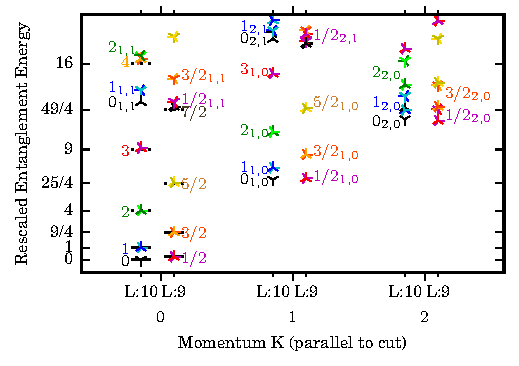
\includegraphics[width=\columnwidth]{EEIdentify.pdf}
	\caption{The identification of the states $j_{-n}\ket{e, m=0}$ in the spectrum of the soft-core boson entanglement Hamiltonian. The label $e$ gives the U(1) charge. The labels $n$, $\bar{n}$ label the levels in the right or left-moving sectors of the Kac-Moody algebra.  The best estimate for the Luttinger parameter is $\kappa = 1/6.4$. The label $m$ is 0 for all states shown - however, the primary states $\ket{e, m=\pm 1}$ can be seen centered around momentum $\pi$.}
	\label{fig:primaries}
\end{figure}



\subsection{Symmetry action on the edge}

\begin{figure}[H]
    \centering
    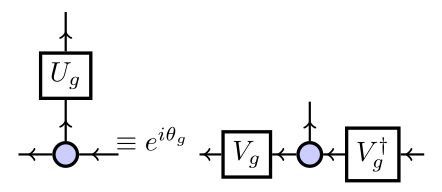
\includegraphics[width=0.6\columnwidth]{group_sym.png}
\end{figure}


\begin{figure}[H]
    \centering
    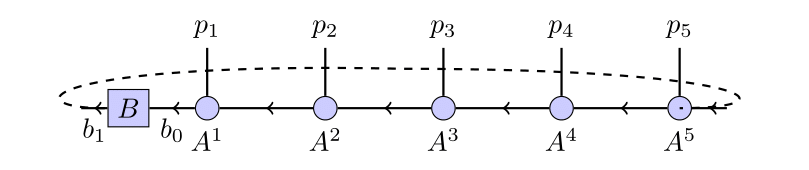
\includegraphics[width=\columnwidth]{mpsbc.png}
\end{figure}

\begin{tabular*}{\columnwidth}{@{\extracolsep{\stretch{1}}}*{5}{r}@{}}
\toprule
$\mathbf{G}$ & $\mathbf{U_g}$ & $\mathbf{\theta_g}$ & $\mathbf{V_g}$ &$\mathbf{V_g V^*_g}$ \\
\midrule
 $U(1)$ & & & & \\
 $\mathcal{\pi}$ & & & & \\
 $\mathcal{I}$ & & & & \\
 $\mathcal{\pi} \mathcal{I}$ & & & & \\
\bottomrule
\end{tabular*}

Since 
$$  
V_{\mathcal{\pi} \mathcal{I}} V_{\mathcal{\pi} \mathcal{I}}^* = -I \text{\quad or \quad } V_{\mathcal{\pi}} V_{\mathcal{I}} = - V_{\mathcal{I}} V_{\mathcal{\pi}},
$$ 

the representation is in the nontrivial class of 

$$
H^2(\mathbb{Z}_2 \times \mathbb{Z}_2^{\mathcal{I}}; U(1)) = \mathbb{Z}_2.
$$